
 \documentclass[a4paper,12pt]{article}
 %%%%%%%%%%%%%%%%%%%%%%%%%%%%%%%%%%%%%%%%%%%%%%%%%%%%%%%%%%%%%%%%%%%%%%%%%%%%%%%%%%%%%%%%%%%%%%%%%%%%%%%%%%%%%%%%%%%%%%%%%%%%%%%%%%%%%%%%%%%%%%%%%%%%%%%%%%%%%%%%%%%%%%%%%%%%%%%%%%%%%%%%%%%%%%%%%%%%%%%%%%%%%%%%%%%%%%%%%%%%%%%%%%%%%%%%%%%%%%%%%%%%%%%%%%%%
 \usepackage{eurosym}
 \usepackage{vmargin}
 \usepackage{amsmath}
 \usepackage{multicol}
 \usepackage{graphics}
 \usepackage{enumerate}
 \usepackage{epsfig}
 \usepackage{framed}
 \usepackage{subfigure}
 \usepackage{fancyhdr}
 
 \setcounter{MaxMatrixCols}{10}
 %TCIDATA{OutputFilter=LATEX.DLL}
 %TCIDATA{Version=5.00.0.2570}
 %TCIDATA{<META NAME="SaveForMode" CONTENT="1">}
 %TCIDATA{LastRevised=Wednesday, February 23, 2011 13:24:34}
 %TCIDATA{<META NAME="GraphicsSave" CONTENT="32">}
 %TCIDATA{Language=American English}
 
 %\pagestyle{fancy}
 \setmarginsrb{20mm}{0mm}{20mm}{25mm}{12mm}{11mm}{0mm}{11mm}
 %\lhead{MA4413 2013} \rhead{Mr. Kevin O'Brien}
 
 
 \begin{document}
 	\tableofcontents
\newpage


\subsection{Diagnostic Plots for LME models}

Pinheiro and Bates provide some insight into how to compute and interpret model diagnostic plots for lme models. Unfortunately this aspect of LME theory is not as expansive as the corresponding body of work for Linear Models.

When the \texttt{plot} function calls the model object, the residual plot is produced.





\begin{framed}
\begin{verbatim}
plot(JS.roy1, which=c(1) )
\end{verbatim}
\end{framed}


\begin{figure}[h!]
	\centering
	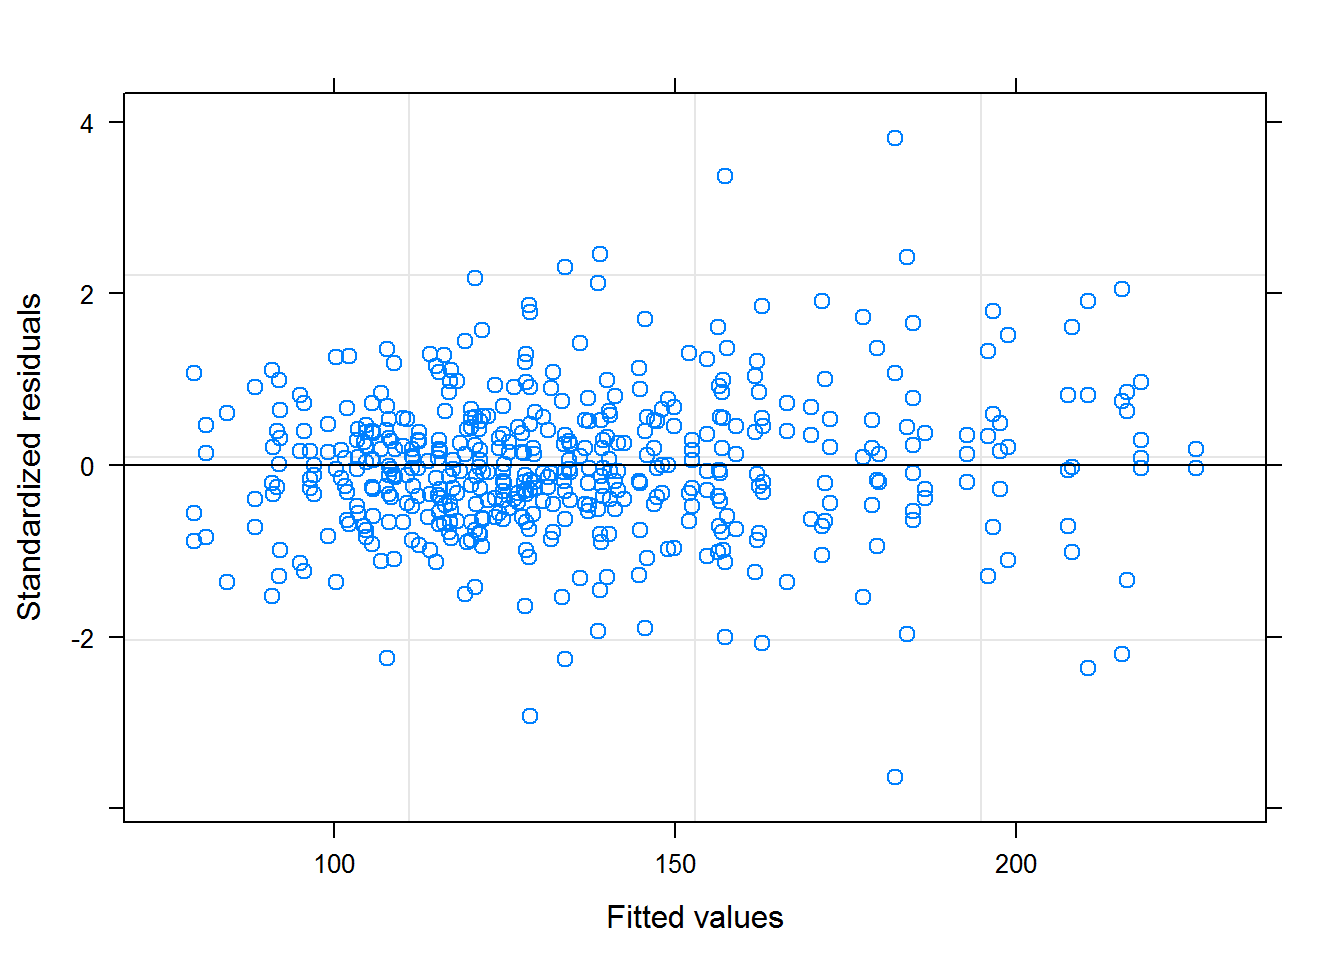
\includegraphics[width=0.9\linewidth]{images/ResidPlot1}
	\caption{}
	\label{fig:ResidPlot1}
\end{figure}
LME models assume that the residuals of the model are normally distributed. A Normal probability plot can be constructed to check this assumption. Commonly used \texttt{R} commands cabbe used to construct the plot.
\newpage

\begin{framed}
	\begin{verbatim}
qqnorm(resid(JS.roy1),pch="*",col="red")
qqline(resid(JS.roy1),col="blue")
	\end{verbatim}
\end{framed}




\begin{figure}[h!]
	\centering
	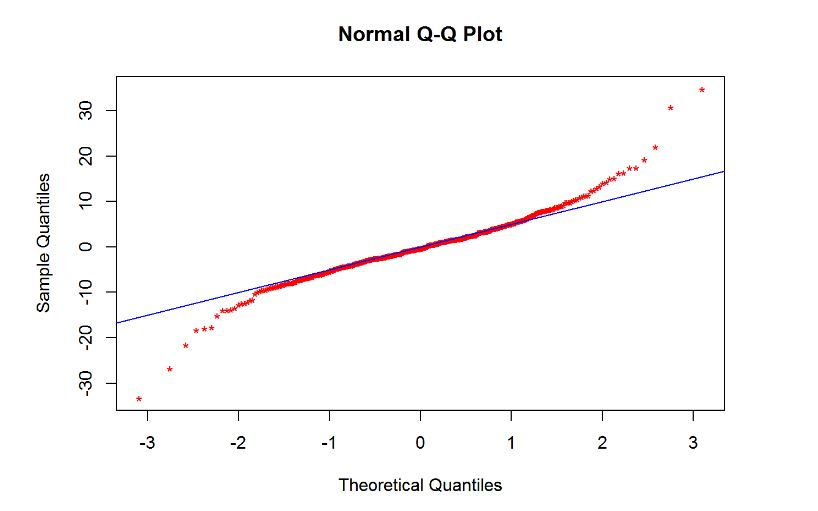
\includegraphics[width=0.7\linewidth]{images/Resid-newplot}
	\caption{}
	\label{fig:Resid-newplot}
\end{figure}

\begin{framed}
\begin{verbatim}
table(dat$method[1:255])
## 
##   J   S 
## 255   0
table(dat$method[256:510])
## 
##   J   S 
##   0 255
\end{verbatim}	
\end{framed}



\newpage

\subsubsection{Checking the Assumption by Method}

\begin{framed}
\begin{verbatim}
par(mfrow=c(1,2))
qqnorm((resid(JS.roy1)[1:255]),
      pch="*",col="red",
      ylim=c(-40,40),
      main="Method J")
qqline(resid(JS.roy1)[1:255],col="blue")
qqnorm((resid(JS.roy1)[256:510]),
      pch="*",col="red",
      ylim=c(-40,40),
      main="Method S")
qqline(resid(JS.roy1)[256:510],col="blue")
par(mfrow=c(1,1))
\end{verbatim}	
\end{framed}


\begin{figure}[h!]
	\centering
	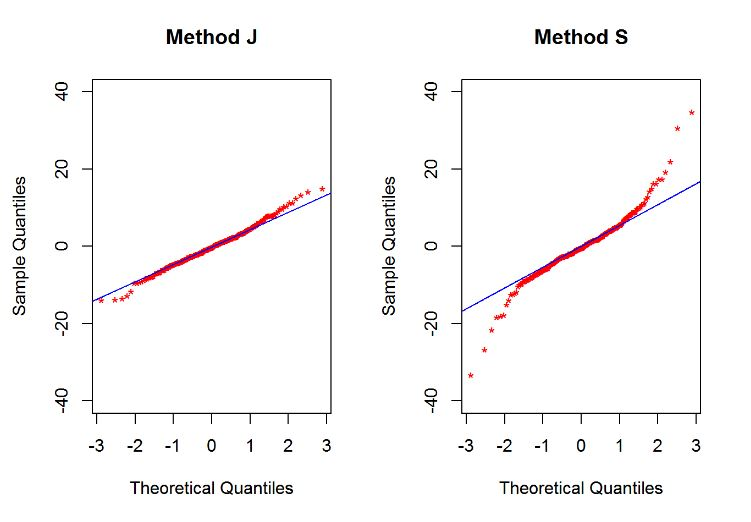
\includegraphics[width=1.1\linewidth]{images/Resid-newplot2}
	\caption{}
	\label{fig:Resid-newplot2}
\end{figure}


\begin{figure}[h!]
	\centering
	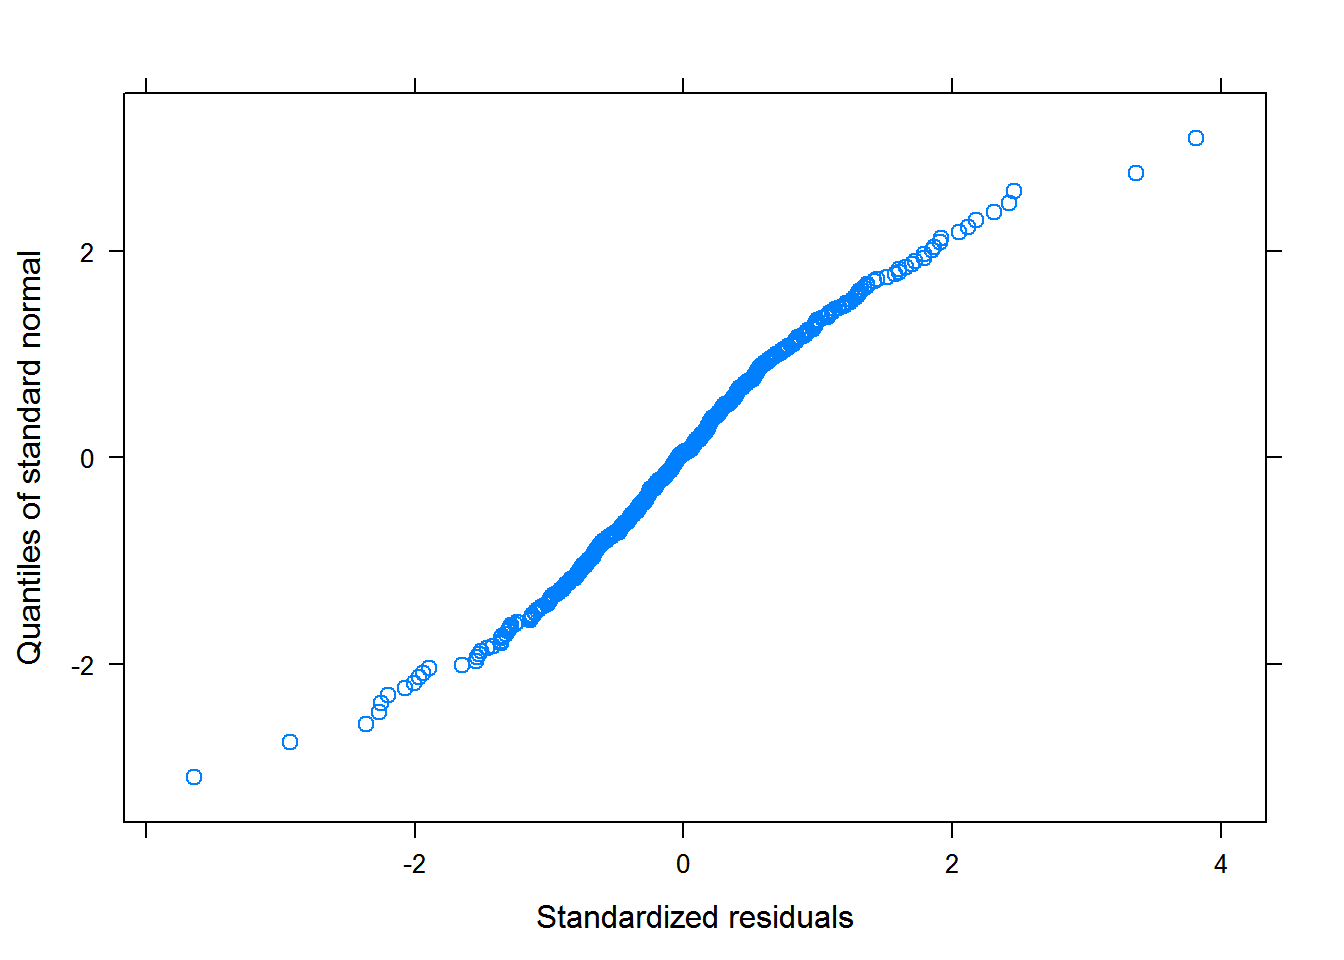
\includegraphics[width=0.9\linewidth]{images/ResidPlot3}
	\caption{}
	\label{fig:ResidPlot3}
\end{figure}

This code will allow you to make QQ plots for each level of the random effects.  LME models assume that not only the within-cluster residuals are normally distributed, but that each level of the random effects are as well. Depending on the model, you can vary the level from 0, 1, 2 and so on
\begin{framed}
\begin{verbatim}
qqnorm(JS.roy1, ~ranef(.))
\end{verbatim}
\end{framed}


\begin{framed}
\begin{verbatim}
qqnorm(JS.roy1, ~ranef(.,levels=1)
\end{verbatim}
\end{framed}
\begin{figure}[h!]
\centering
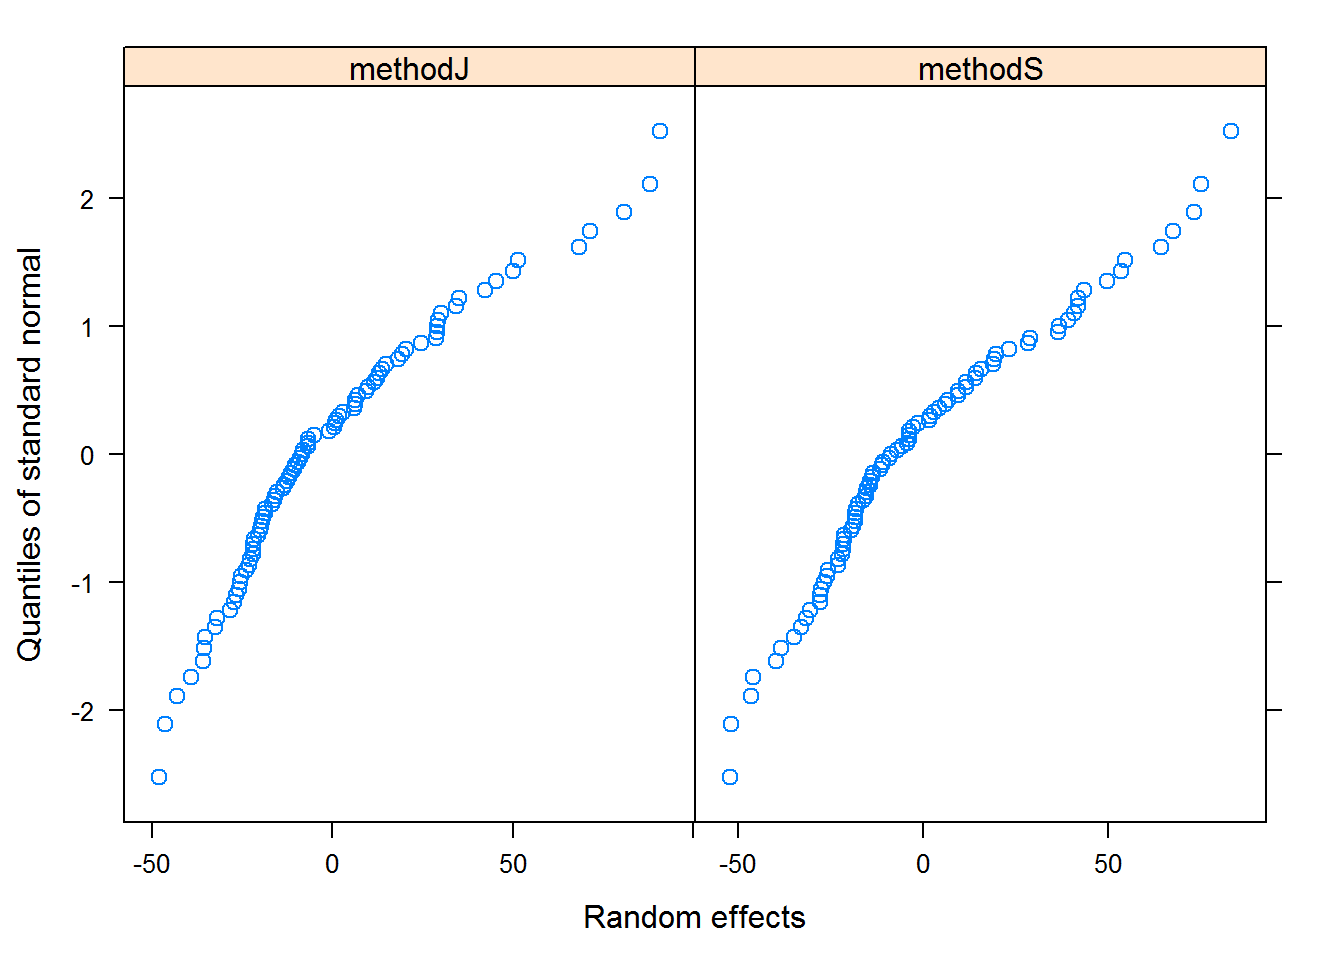
\includegraphics[width=0.9\linewidth]{images/ResidPlot2}
\caption{}
\label{fig:ResidPlot2}
\end{figure}

\end{document}

